\begin{knitrout}
\definecolor{shadecolor}{rgb}{0.969, 0.969, 0.969}\color{fgcolor}\begin{figure}

{\centering 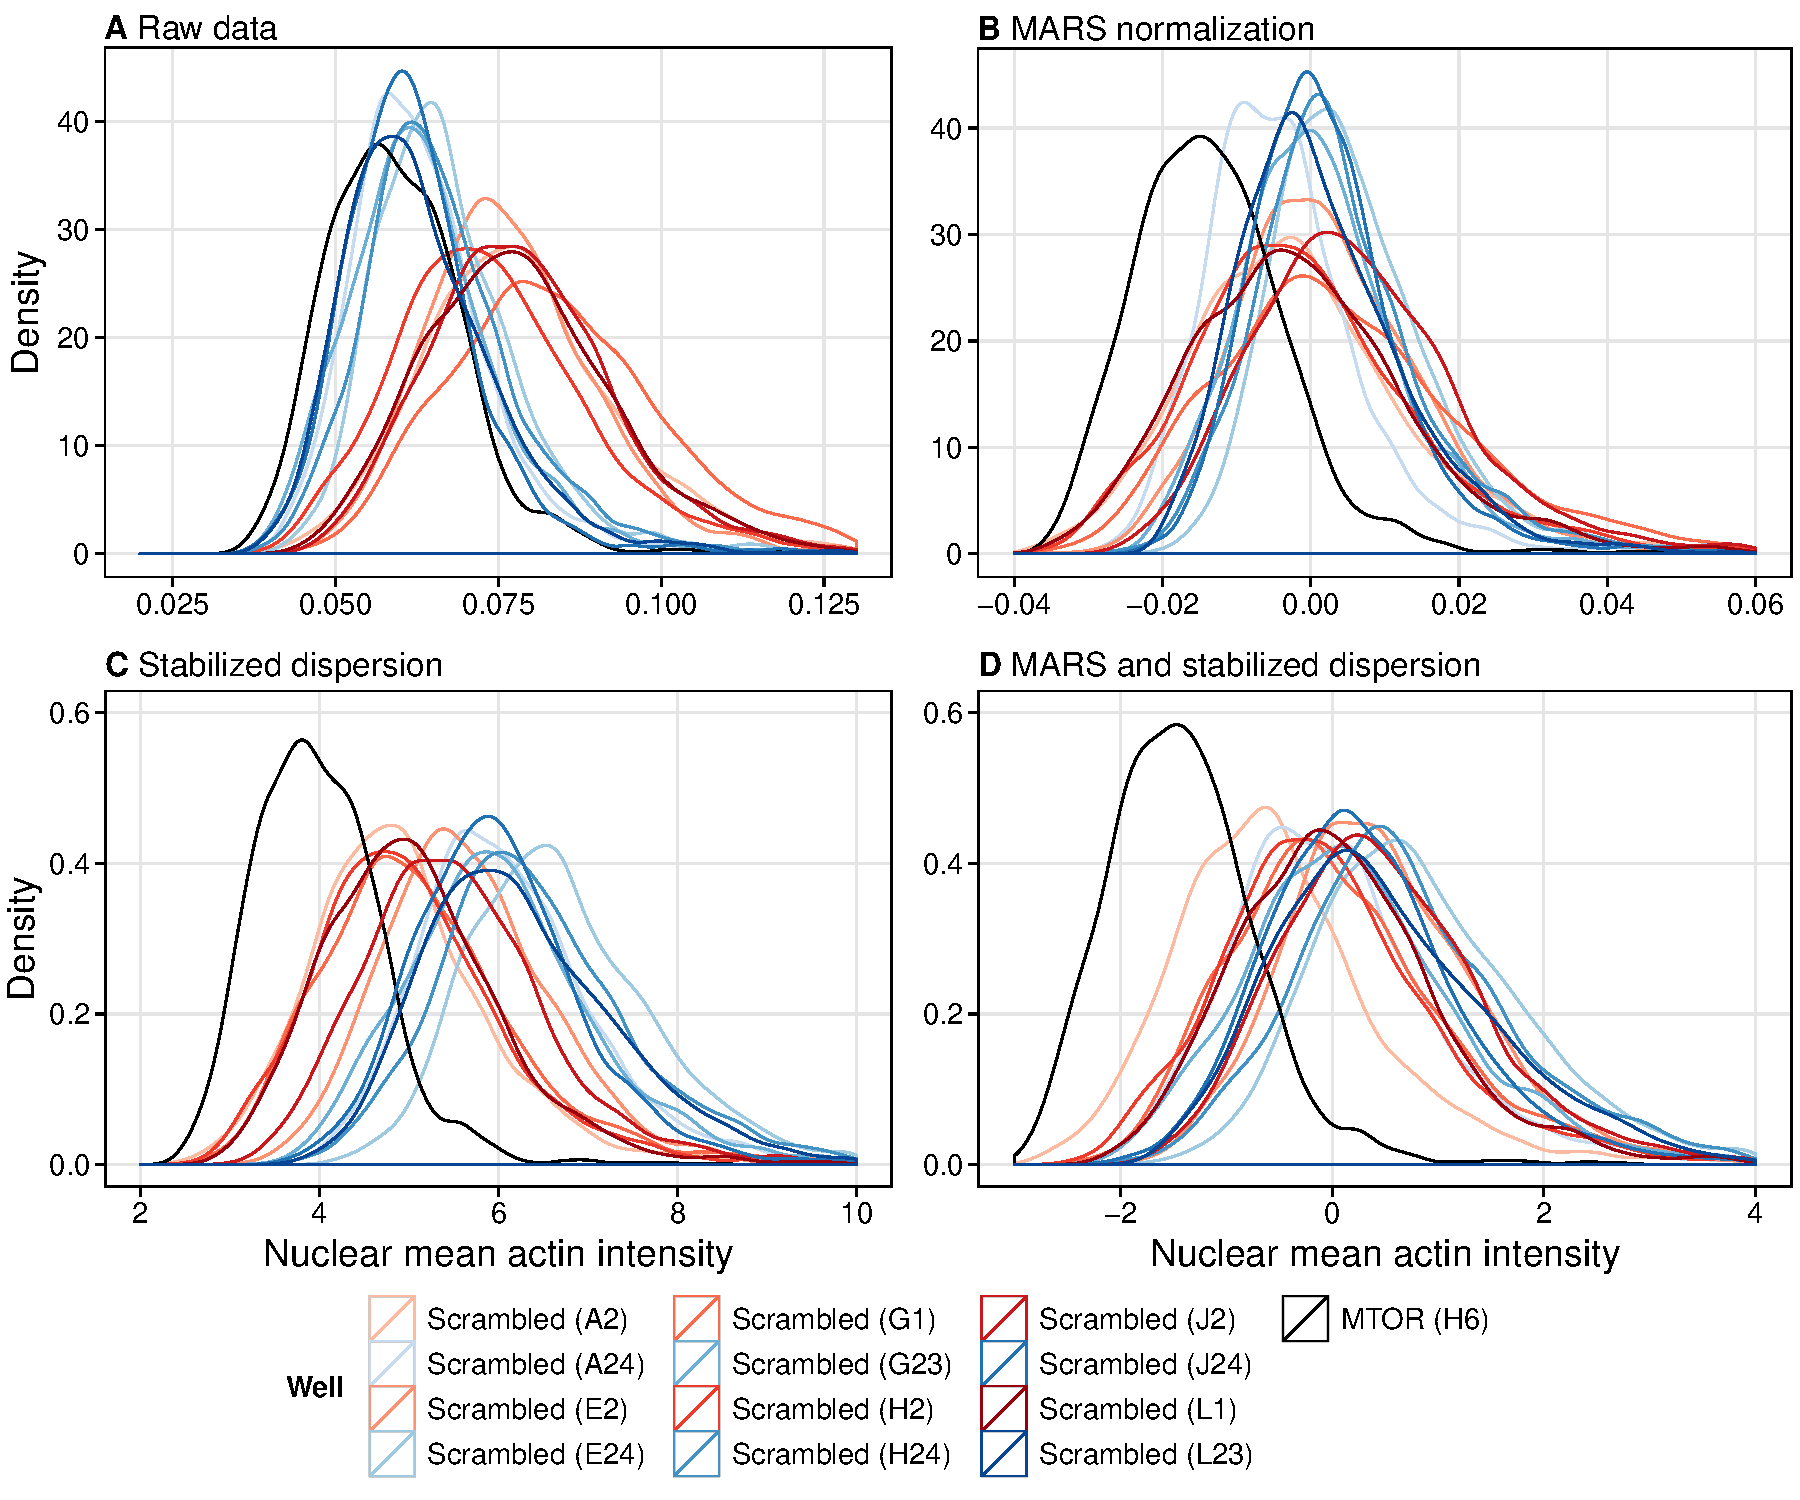
\includegraphics[width=\maxwidth]{figures/R/normalization-data-actin-normalization-1} 

}

\caption[Effects of normalization schemes visualized through density plots.]{In order to provide intuitive access to how normalization affects the data, four density plots are reproduced, using mean nuclear actin intensity for \ACRshort{mtor} and scrambled wells of plate J110-2D. The top left plot represents the raw data and both a clear separation of two groups of scrambled wells (corresponding to early and late column wells) can be recognized, as well as the issue that differences between \ACRshort{mtor} wells and scrambled wells appear no larger than differences among scrambled wells (A). Moving to the right partially recovers some issues, as scrambled distributions now all roughly share the same center (B), while moving downwards improves the problem of varying dispersion with respect to scrambled grouping (C). Finally, bottom right represents a combination of both schemes, yielding the best result in that scrambled wells become more similar while differences to \ACRshort{mtor} are retained (D).}\label{fig:data-actin-normalization}
\end{figure}


\end{knitrout}
